\documentclass{standalone}
\usepackage{placeins}
\begin{document}


\section{Design}
Sparkling Water is designed to be executed as a regular Spark application. It provides a way to initialize H2O services on each node in the Spark cluster and access data stored in data structures of Spark and H2O.

Since Sparkling Water is primarily designed as Spark application, it is launched
inside a Spark executor created after submitting the application. At this
point, H2O starts services, including distributed key-value (K/V) store and memory manager, and orchestrates them into a cloud. The topology of the created cloud replicates the topology of the underlying Spark cluster.

\begin{figure}[h!]
	\centering
	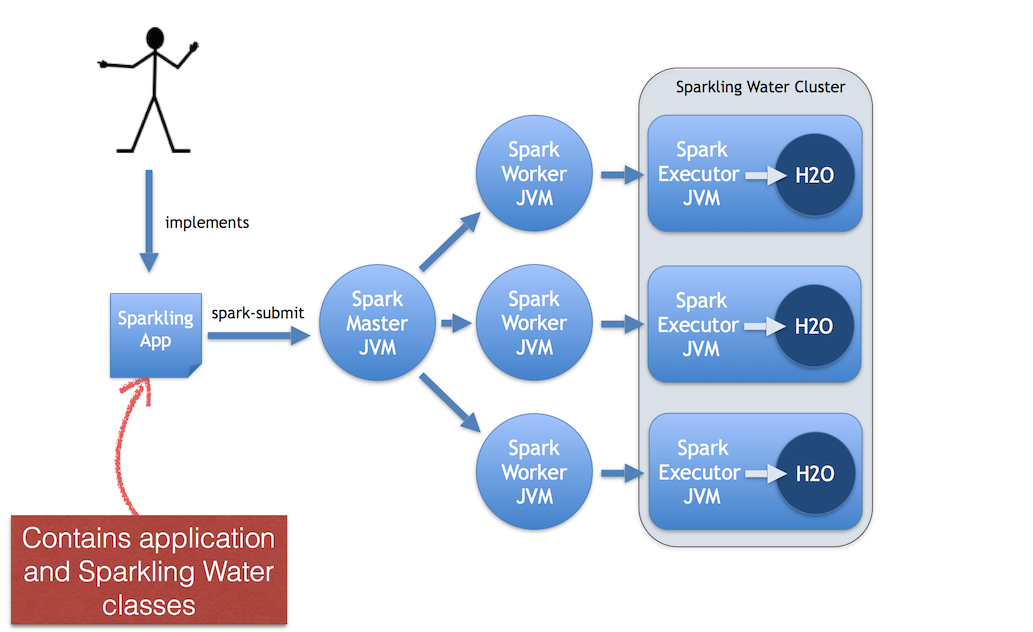
\includegraphics[scale=0.6]{sw/images/Topology.png}
	\caption{Sparkling Water design depicting deployment of the Sparkling Water application to the standalone Spark cluster.}
\end{figure}


\subsection{Data Sharing between Spark and H2O}

Sparkling Water enables transformation between different types of RDDs and H2O's \texttt{H2OFrame}, and vice versa.

When converting from an \texttt{H2OFrame} to an RDD, a wrapper is created around the \texttt{H2OFrame} to provide an RDD-like API. In this case,  data is not duplicated but served directly from the underlying \texttt{H2OFrame}.

Converting from an RDD/DataFrame to an \texttt{H2OFrame} requires data duplication because it transfers data from the RDD storage into \texttt{H2OFrame}. However, data stored in an \texttt{H2OFrame} is heavily compressed and does not need to be preserved in RDD.

\begin{figure}[h!]
	\centering
	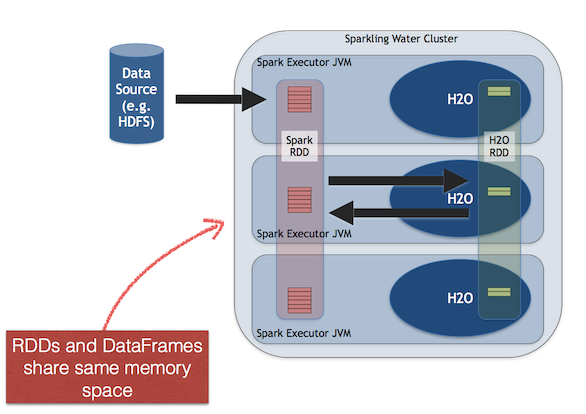
\includegraphics[scale=1]{sw/images/DataShare.png}
	\caption{Sharing between Spark and H2O inside an executor JVM.}
\end{figure}


\subsection{Provided Primitives}

Sparkling Water provides several primitives (for more information, refer to Table~\ref{tab:primitives}). Before using H2O algorithms and data structures, the first step is to create and start the \texttt{H2OContext} instance using the \texttt{val hc = new H2OContext(sc).start()} call. 

The \texttt{H2OContext} contains the necessary information for running H2O services and exposes methods for data transformation between the Spark RDD or \texttt{DataFrame} and the \texttt{H2OFrame}. Starting \texttt{H2OContext} involves a distributed operation that contacts all accessible Spark executor nodes and initializes H2O services (such as the key-value store and RPC) inside the executors' JVMs.

When \texttt{H2OContext} is running, H2O data structures and algorithms can be manipulated. The key data structure is \texttt{H2OFrame}, which represents a distributed table composed of vectors. A new \texttt{H2OFrame} can be created using one of the following methods:
\begin{itemize}
	\item loading a cluster local file (a file located on each node of the cluster):
\begin{lstlisting}[style=Scala]
val h2oFrame = new H2OFrame(new File("/data/iris.csv"))
\end{lstlisting}
	\item loading a file from HDFS/S3/S3N/S3A:
\begin{lstlisting}[style=Scala]
val h2oFrame = new H2OFrame(URI.create("hdfs://data/iris.csv"))
\end{lstlisting}
	\item loading multiple files from HDFS/S3/S3N/S3A:
\begin{lstlisting}[style=Scala]
val h2oFrame = new H2OFrame(URI.create("hdfs://data/iris/01.csv"), URI.create("hdfs://data/iris/02.csv"))
\end{lstlisting}
	\item transforming Spark RDD or \texttt{DataFrame}:
\begin{lstlisting}[style=Scala]
val h2oFrame = h2oContext.asH2OFrame(rdd)
\end{lstlisting}
	\item referencing existing \texttt{H2OFrame} by its key
\begin{lstlisting}[style=Scala]
val h2oFrame = new H2OFrame("iris.hex")
\end{lstlisting}		
\end{itemize}

\begin{table}[!ht]
\centering
%\begin{adjustbox}{width=\textwidth} %resizes table to text width
%\setlength{\tabcolsep}{2pt} %narrow column separation
\begin{tabular}{c c p{5.2cm}}
%\begin{tabularx}{\textwidth}{l l p{5.2cm}}
\toprule
Concept & API Representation & Description \\
\midrule
H2O Context & \texttt{H2OContext} & Contains the
H2O state and provides primitives to publish \texttt{RDD} as \texttt{H2OFrame} and
vice versa. Follows design principles of Spark primitives such as
\texttt{SparkContext} or \texttt{SQLContext}. \\ \addlinespace
%\small{(Full name: \small{\texttt{org.apache.spark.\break h2o.H2OContext}}}) \\  \addlinespace

H2O Entry Point & \texttt{water.H2O} & Represents the entry point for accessing
H2O services. Contains information about running H2O services, including a list of
nodes and the status of the distributed K/V datastore. \\  \addlinespace

H2O Frame &  \small{\texttt{water.fvec.H2OFrame}} & A data structure 
representing a table of values. The table is column-based and provides column and
row accessors. \\  \addlinespace

H2O Algorithm & package \texttt{hex} & Represents the H2O machine learning
algorithms library, including DeepLearning, GBM, GLM, DRF, and other
algorithms. \\

\bottomrule
\end{tabular} 
%\end{tabularx}
\caption{Sparkling Water primitives}
\label{tab:primitives}
\end{table}

\pagebreak
When the \texttt{H2OContext} is running, any H2O algorithm can be called. Most of provided algorithms are located in the \texttt{hex} package. Calling an algorithm is composed of two steps:

\begin{itemize}
	\item Specifying parameters:
\begin{lstlisting}[style=Scala]
val train: H2OFrame = new H2OFrame(new File("prostate.csv"))
val gbmParams = new GBMParameters()
gbmParams._train = train
gbmParams._response_column = 'CAPSULE
gbmParams._ntrees = 10
\end{lstlisting}

	\item Creating the model builder and launching computations. The \texttt{trainModel} method is non-blocking and returns a job representing the computation.
\begin{lstlisting}[style=Scala]
val gbmModel = new GBM(gbmParams).trainModel.get
\end{lstlisting}
\end{itemize}

\end{document}
